\documentclass[11pt,a4paper]{article}

% Packages
\usepackage[utf8]{inputenc}
\usepackage[T1]{fontenc}
\usepackage{geometry}
\usepackage{graphicx}
\usepackage{tikz}
\usepackage{xcolor}
\usepackage{listings}
\usepackage{hyperref}
\usepackage{booktabs}
\usepackage{enumitem}
\usepackage{fancyhdr}
\usepackage{titlesec}
\usepackage{float}
\usepackage{subcaption}
\usepackage{amsmath}
\usepackage{algorithm}
\usepackage{algpseudocode}

% TikZ libraries
\usetikzlibrary{shapes.geometric, arrows.meta, positioning, fit, backgrounds, calc, decorations.pathreplacing}

% Page setup
\geometry{margin=1in}

% Colors
\definecolor{codegreen}{rgb}{0,0.6,0}
\definecolor{codegray}{rgb}{0.5,0.5,0.5}
\definecolor{codepurple}{rgb}{0.58,0,0.82}
\definecolor{backcolour}{rgb}{0.95,0.95,0.92}
\definecolor{darkblue}{RGB}{26,82,118}
\definecolor{lightblue}{RGB}{174,214,241}
\definecolor{darkgreen}{RGB}{39,174,96}
\definecolor{lightgreen}{RGB}{171,235,198}
\definecolor{darkorange}{RGB}{230,126,34}
\definecolor{lightorange}{RGB}{250,215,160}
\definecolor{darkred}{RGB}{192,57,43}
\definecolor{lightred}{RGB}{245,183,177}

% Code listing style
\lstdefinestyle{mystyle}{
    backgroundcolor=\color{backcolour},
    commentstyle=\color{codegreen},
    keywordstyle=\color{darkblue}\bfseries,
    numberstyle=\tiny\color{codegray},
    stringstyle=\color{codepurple},
    basicstyle=\ttfamily\footnotesize,
    breakatwhitespace=false,
    breaklines=true,
    captionpos=b,
    keepspaces=true,
    numbers=left,
    numbersep=5pt,
    showspaces=false,
    showstringspaces=false,
    showtabs=false,
    tabsize=2,
    frame=single,
    rulecolor=\color{codegray}
}
\lstset{style=mystyle}

% Header/Footer
\pagestyle{fancy}
\fancyhf{}
\fancyhead[L]{\small VPR Deployment Guide}
\fancyhead[R]{\small CMU-Africa}
\fancyfoot[C]{\thepage}

% Hyperref setup
\hypersetup{
    colorlinks=true,
    linkcolor=darkblue,
    filecolor=darkblue,
    urlcolor=darkblue,
}

% Title formatting
\titleformat{\section}{\Large\bfseries\color{darkblue}}{\thesection}{1em}{}
\titleformat{\subsection}{\large\bfseries\color{darkblue!80}}{\thesubsection}{1em}{}

\begin{document}

% Title Page
\begin{titlepage}
    \centering
    \vspace*{2cm}

    {\Huge\bfseries Visual Place Recognition\\[0.3cm] Practical Deployment Guide\par}

    \vspace{1.5cm}

    {\Large Live Testing with Mobile Phone Camera\par}

    \vspace{2cm}

    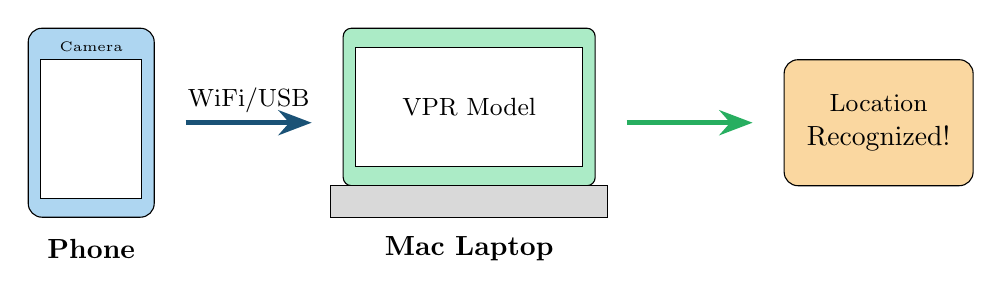
\begin{tikzpicture}[scale=0.8]
        % Phone
        \draw[fill=lightblue, rounded corners=5pt] (-4,0) rectangle (-2,3);
        \draw[fill=white] (-3.8,0.3) rectangle (-2.2,2.5);
        \node at (-3,2.7) {\tiny Camera};
        \node at (-3,-0.5) {\textbf{Phone}};

        % Arrow
        \draw[-{Stealth}, line width=2pt, darkblue] (-1.5,1.5) -- (0.5,1.5);
        \node[above] at (-0.5,1.5) {\small WiFi/USB};

        % Laptop
        \draw[fill=lightgreen, rounded corners=3pt] (1,0.5) rectangle (5,3);
        \draw[fill=white] (1.2,0.8) rectangle (4.8,2.7);
        \draw[fill=gray!30] (0.8,0) rectangle (5.2,0.5);
        \node at (3,1.75) {\small VPR Model};
        \node at (3,-0.5) {\textbf{Mac Laptop}};

        % Output
        \draw[-{Stealth}, line width=2pt, darkgreen] (5.5,1.5) -- (7.5,1.5);

        % Result
        \draw[fill=lightorange, rounded corners=5pt] (8,0.5) rectangle (11,2.5);
        \node[align=center] at (9.5,1.5) {\small Location\\Recognized!};
    \end{tikzpicture}

    \vspace{2cm}

    {\Large\textbf{Authors}\par}
    \vspace{0.5cm}
    {\large Rhoda Ojetola \\ Peter Adeyemo \\ Samuel Olusola\par}

    \vspace{1.5cm}

    {\large MS in Engineering Artificial Intelligence\\
    Computer Vision Lab\\
    Carnegie Mellon University Africa\\[0.5cm]
    March 2026\par}

\end{titlepage}

% Table of Contents
\tableofcontents
\newpage

% ============================================================================
\section{Introduction}
% ============================================================================

\subsection{What is Visual Place Recognition?}

Visual Place Recognition (VPR) is the task of recognizing a previously visited location using images. Given a database of reference images from known locations and query images from unknown locations, VPR systems determine which query images correspond to which database images.

\begin{figure}[H]
    \centering
    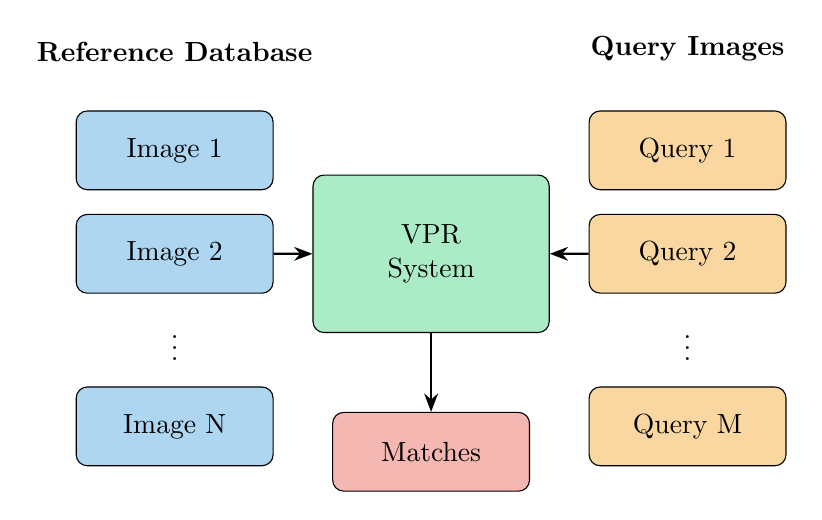
\begin{tikzpicture}[
        node distance=1.5cm,
        box/.style={rectangle, draw, rounded corners, minimum width=2.5cm, minimum height=1cm, align=center},
        arrow/.style={-{Stealth}, thick}
    ]
        % Database side
        \node[box, fill=lightblue] (db1) {Image 1};
        \node[box, fill=lightblue, below=0.3cm of db1] (db2) {Image 2};
        \node[below=0.2cm of db2] (dots1) {$\vdots$};
        \node[box, fill=lightblue, below=0.2cm of dots1] (dbn) {Image N};

        \node[above=0.5cm of db1, font=\bfseries] {Reference Database};

        % Query side
        \node[box, fill=lightorange, right=4cm of db1] (q1) {Query 1};
        \node[box, fill=lightorange, below=0.3cm of q1] (q2) {Query 2};
        \node[below=0.2cm of q2] (dots2) {$\vdots$};
        \node[box, fill=lightorange, below=0.2cm of dots2] (qm) {Query M};

        \node[above=0.5cm of q1, font=\bfseries] {Query Images};

        % VPR System
        \node[box, fill=lightgreen, minimum width=3cm, minimum height=2cm] (vpr) at ($(db2)!0.5!(q2)$) {VPR\\System};

        % Arrows
        \draw[arrow] (db2.east) -- (vpr.west);
        \draw[arrow] (q2.west) -- (vpr.east);

        % Output
        \node[box, fill=lightred, below=1cm of vpr] (out) {Matches};
        \draw[arrow] (vpr.south) -- (out.north);

    \end{tikzpicture}
    \caption{Visual Place Recognition: matching query images to a reference database.}
\end{figure}

\subsection{Applications}

\begin{itemize}
    \item \textbf{Robot Localization}: Determining a robot's position in a mapped environment
    \item \textbf{Loop Closure Detection}: Recognizing revisited locations in SLAM
    \item \textbf{Image Retrieval}: Finding similar images in large databases
    \item \textbf{Autonomous Navigation}: Enabling GPS-denied localization
\end{itemize}

\subsection{Challenges}

\begin{itemize}
    \item \textbf{Illumination Changes}: Day vs. night recognition
    \item \textbf{Seasonal Variations}: Same place across different seasons
    \item \textbf{Viewpoint Changes}: Different camera angles and positions
    \item \textbf{Efficiency}: Real-time performance with large databases
\end{itemize}

\newpage
% ============================================================================
\section{System Architecture}
% ============================================================================

\subsection{Overview}

The VPR system operates in two phases: an \textbf{offline phase} for building the reference database, and an \textbf{online phase} for real-time localization.

\begin{figure}[H]
    \centering
    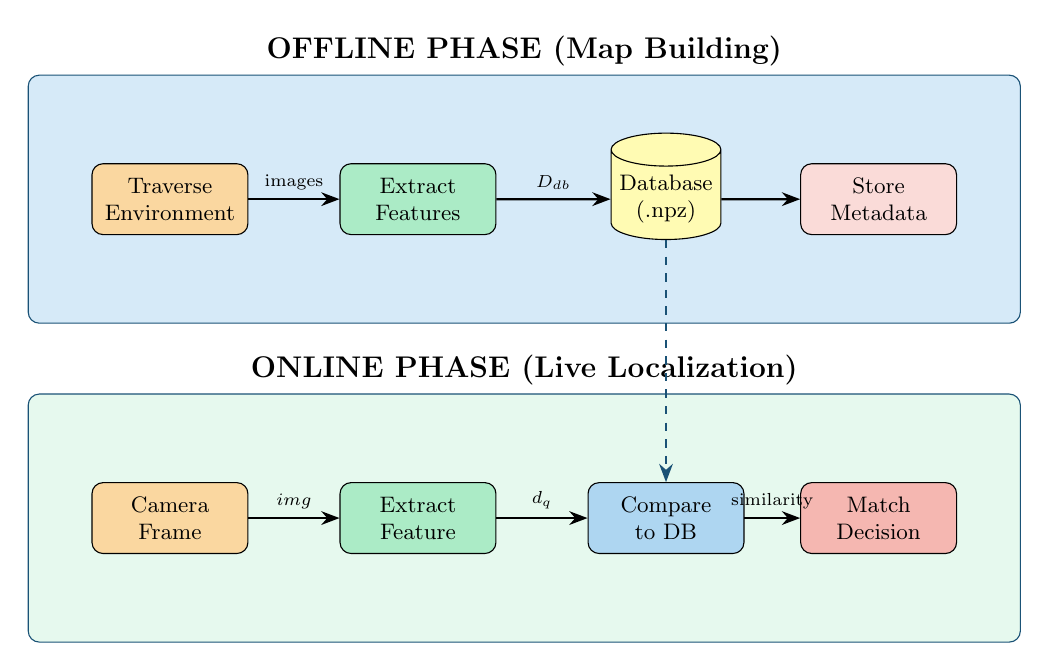
\begin{tikzpicture}[
        scale=0.9,
        transform shape,
        phase/.style={rectangle, draw=darkblue, fill=lightblue!50, rounded corners, minimum width=14cm, minimum height=3.5cm},
        block/.style={rectangle, draw, rounded corners, minimum width=2.2cm, minimum height=1cm, align=center, font=\small},
        data/.style={cylinder, draw, shape border rotate=90, minimum width=1.5cm, minimum height=1cm, aspect=0.3, align=center, font=\small},
        arrow/.style={-{Stealth}, thick}
    ]
        % Offline Phase
        \node[phase, label={[font=\bfseries\large]above:OFFLINE PHASE (Map Building)}] (offline) at (0,4) {};

        \node[block, fill=lightorange] (traverse) at (-5,4) {Traverse\\Environment};
        \node[block, fill=lightgreen] (extract1) at (-1.5,4) {Extract\\Features};
        \node[data, fill=yellow!30] (dbstore) at (2,4) {Database\\(.npz)};
        \node[block, fill=lightred!50] (meta) at (5,4) {Store\\Metadata};

        \draw[arrow] (traverse) -- node[above, font=\scriptsize] {images} (extract1);
        \draw[arrow] (extract1) -- node[above, font=\scriptsize] {$D_{db}$} (dbstore);
        \draw[arrow] (dbstore) -- (meta);

        % Online Phase
        \node[phase, fill=lightgreen!30, label={[font=\bfseries\large]above:ONLINE PHASE (Live Localization)}] (online) at (0,-0.5) {};

        \node[block, fill=lightorange] (camera) at (-5,-0.5) {Camera\\Frame};
        \node[block, fill=lightgreen] (extract2) at (-1.5,-0.5) {Extract\\Feature};
        \node[block, fill=lightblue] (compare) at (2,-0.5) {Compare\\to DB};
        \node[block, fill=lightred] (decision) at (5,-0.5) {Match\\Decision};

        \draw[arrow] (camera) -- node[above, font=\scriptsize] {$img$} (extract2);
        \draw[arrow] (extract2) -- node[above, font=\scriptsize] {$d_q$} (compare);
        \draw[arrow] (compare) -- node[above, font=\scriptsize] {similarity} (decision);

        % Connection between phases
        \draw[arrow, dashed, darkblue] (dbstore.south) -- ++(0,-1) -| (compare.north);

    \end{tikzpicture}
    \caption{Two-phase VPR system architecture.}
\end{figure}

\subsection{Detailed Pipeline}

\begin{figure}[H]
    \centering
    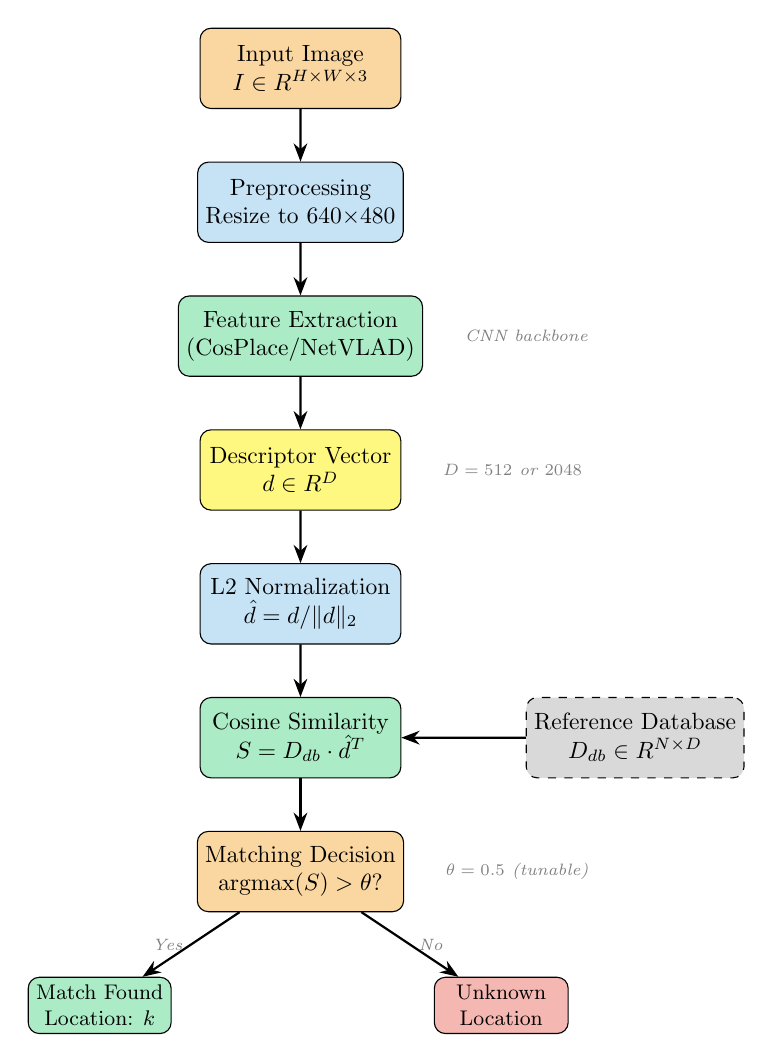
\begin{tikzpicture}[
        scale=0.85,
        transform shape,
        block/.style={rectangle, draw, rounded corners, minimum width=3cm, minimum height=1.2cm, align=center},
        smallblock/.style={rectangle, draw, rounded corners, minimum width=2cm, minimum height=0.8cm, align=center, font=\small},
        arrow/.style={-{Stealth}, thick},
        note/.style={font=\scriptsize\itshape, text=gray}
    ]
        % Input
        \node[block, fill=lightorange] (input) at (0,0) {Input Image\\$I \in \mathbb{R}^{H \times W \times 3}$};

        % Preprocessing
        \node[block, fill=lightblue!70] (preprocess) at (0,-2) {Preprocessing\\Resize to 640$\times$480};

        % Feature Extraction
        \node[block, fill=lightgreen] (extract) at (0,-4) {Feature Extraction\\(CosPlace/NetVLAD)};

        % Descriptor
        \node[block, fill=yellow!50] (descriptor) at (0,-6) {Descriptor Vector\\$d \in \mathbb{R}^{D}$};

        % Normalization
        \node[block, fill=lightblue!70] (normalize) at (0,-8) {L2 Normalization\\$\hat{d} = d / \|d\|_2$};

        % Similarity
        \node[block, fill=lightgreen] (similarity) at (0,-10) {Cosine Similarity\\$S = D_{db} \cdot \hat{d}^T$};

        % Database
        \node[block, fill=gray!30, dashed] (database) at (5,-10) {Reference Database\\$D_{db} \in \mathbb{R}^{N \times D}$};

        % Decision
        \node[block, fill=lightorange] (decision) at (0,-12) {Matching Decision\\$\text{argmax}(S) > \theta$?};

        % Outputs
        \node[smallblock, fill=lightgreen] (match) at (-3,-14) {Match Found\\Location: $k$};
        \node[smallblock, fill=lightred] (nomatch) at (3,-14) {Unknown\\Location};

        % Arrows
        \draw[arrow] (input) -- (preprocess);
        \draw[arrow] (preprocess) -- (extract);
        \draw[arrow] (extract) -- (descriptor);
        \draw[arrow] (descriptor) -- (normalize);
        \draw[arrow] (normalize) -- (similarity);
        \draw[arrow] (database) -- (similarity);
        \draw[arrow] (similarity) -- (decision);
        \draw[arrow] (decision) -- node[left, note] {Yes} (match);
        \draw[arrow] (decision) -- node[right, note] {No} (nomatch);

        % Notes
        \node[note, right=0.5cm of extract] {CNN backbone};
        \node[note, right=0.5cm of descriptor] {$D = 512$ or $2048$};
        \node[note, right=0.5cm of decision] {$\theta = 0.5$ (tunable)};

    \end{tikzpicture}
    \caption{Detailed processing pipeline for a single query image.}
\end{figure}

\newpage
\subsection{Mathematical Formulation}

\subsubsection{Feature Extraction}
Given an image $I$, the feature extractor produces a descriptor vector:
\begin{equation}
    d = f_\theta(I) \in \mathbb{R}^D
\end{equation}
where $f_\theta$ is a neural network (e.g., CosPlace, NetVLAD) with parameters $\theta$.

\subsubsection{Database Construction}
For $N$ reference images $\{I_1, I_2, \ldots, I_N\}$:
\begin{equation}
    D_{db} = \begin{bmatrix} \hat{d}_1^T \\ \hat{d}_2^T \\ \vdots \\ \hat{d}_N^T \end{bmatrix} \in \mathbb{R}^{N \times D}
\end{equation}
where $\hat{d}_i = d_i / \|d_i\|_2$ is the L2-normalized descriptor.

\subsubsection{Similarity Computation}
For a query descriptor $\hat{d}_q$:
\begin{equation}
    S = D_{db} \cdot \hat{d}_q^T \in \mathbb{R}^N
\end{equation}
Each element $S_i$ represents the cosine similarity between the query and reference image $i$.

\subsubsection{Matching Decision}
\begin{equation}
    \text{match} = \begin{cases}
        \text{argmax}(S) & \text{if } \max(S) > \theta \\
        \text{None} & \text{otherwise}
    \end{cases}
\end{equation}

\newpage
% ============================================================================
\section{Hardware Setup}
% ============================================================================

\subsection{Required Equipment}

\begin{table}[H]
    \centering
    \begin{tabular}{lll}
        \toprule
        \textbf{Component} & \textbf{Requirement} & \textbf{Notes} \\
        \midrule
        Phone & Any smartphone with camera & Android or iPhone \\
        Laptop & Mac with Python 3.8+ & GPU optional but faster \\
        Connection & USB cable or WiFi & Same network for WiFi \\
        Storage & 2+ GB free space & For database and models \\
        \bottomrule
    \end{tabular}
    \caption{Hardware requirements for live VPR testing.}
\end{table}

\subsection{Phone-to-Laptop Connection}

\begin{figure}[H]
    \centering
    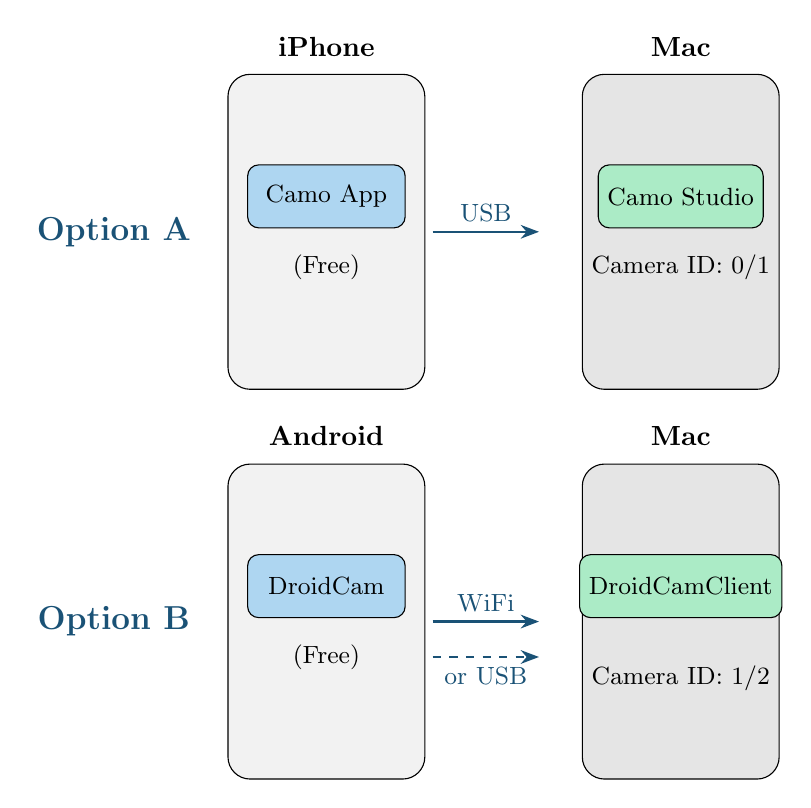
\begin{tikzpicture}[
        scale=0.9,
        device/.style={rectangle, draw, rounded corners=8pt, minimum width=2.5cm, minimum height=4cm, align=center},
        app/.style={rectangle, draw, fill=lightblue, rounded corners, minimum width=2cm, minimum height=0.8cm, font=\small},
        arrow/.style={-{Stealth}, thick, darkblue}
    ]
        % Option A: iPhone
        \node[device, fill=gray!10] (iphone) at (0,0) {};
        \node[above=0.1cm of iphone.north, font=\bfseries] {iPhone};
        \node[app] at (0,0.5) {Camo App};
        \node[font=\small] at (0,-0.5) {(Free)};

        \draw[arrow] (1.5,0) -- node[above, font=\small] {USB} (3,0);

        \node[device, fill=gray!20] (mac1) at (5,0) {};
        \node[above=0.1cm of mac1.north, font=\bfseries] {Mac};
        \node[app, fill=lightgreen] at (5,0.5) {Camo Studio};
        \node[font=\small] at (5,-0.5) {Camera ID: 0/1};

        % Option B: Android
        \node[device, fill=gray!10] (android) at (0,-5.5) {};
        \node[above=0.1cm of android.north, font=\bfseries] {Android};
        \node[app] at (0,-5) {DroidCam};
        \node[font=\small] at (0,-6) {(Free)};

        \draw[arrow] (1.5,-5.5) -- node[above, font=\small] {WiFi} (3,-5.5);
        \draw[arrow, dashed] (1.5,-6) -- node[below, font=\small] {or USB} (3,-6);

        \node[device, fill=gray!20] (mac2) at (5,-5.5) {};
        \node[above=0.1cm of mac2.north, font=\bfseries] {Mac};
        \node[app, fill=lightgreen] at (5,-5) {DroidCam\\Client};
        \node[font=\small] at (5,-6.3) {Camera ID: 1/2};

        % Labels
        \node[font=\bfseries\large, darkblue] at (-3,0) {Option A};
        \node[font=\bfseries\large, darkblue] at (-3,-5.5) {Option B};

    \end{tikzpicture}
    \caption{Two methods for connecting phone camera to Mac laptop.}
\end{figure}

\subsubsection{Option A: iPhone with Camo}
\begin{enumerate}
    \item Install \textbf{Camo} app from the App Store (free version works)
    \item Download Camo Studio for Mac: \url{https://reincubate.com/camo/}
    \item Connect iPhone via USB cable
    \item Open Camo on both devices
    \item iPhone camera appears as webcam (typically camera ID 0 or 1)
\end{enumerate}

\subsubsection{Option B: Android with DroidCam}
\begin{enumerate}
    \item Install \textbf{DroidCam} from Play Store
    \item Download DroidCam client for Mac: \url{https://www.dev47apps.com/}
    \item Connect via USB or WiFi (both devices on same network)
    \item Note the IP address shown in the Android app
    \item Connect from Mac client using the IP address
\end{enumerate}

\newpage
% ============================================================================
\section{Software Setup}
% ============================================================================

\subsection{Directory Structure}

\begin{lstlisting}[language=bash, caption=Required directory structure]
VPR_Tutorial/
|-- live_vpr_test.py          # Main testing script
|-- demo.py                    # Original demo script
|-- requirements.txt           # Python dependencies
|
|-- data/
|   |-- CMUAfrica/
|       |-- day/              # Daytime reference images
|       |   |-- 000.jpg
|       |   |-- 001.jpg
|       |   |-- ...
|       |-- night/            # Nighttime query images
|           |-- 000.jpg
|           |-- 001.jpg
|           |-- ...
|
|-- feature_extraction/       # Feature extractor modules
|-- matching/                 # Matching strategies
|-- evaluation/               # Evaluation metrics
\end{lstlisting}

\subsection{Installation}

\begin{lstlisting}[language=bash, caption=Installation commands]
# Navigate to project directory
cd /path/to/VPR_Tutorial

# Create virtual environment (recommended)
python -m venv venv
source venv/bin/activate

# Install dependencies
pip install -r requirements.txt

# Verify installation
python -c "import cv2; import numpy; print('Ready!')"
\end{lstlisting}

\subsection{Data Preparation}

\begin{lstlisting}[language=bash, caption=Organizing the CMU-Africa dataset]
# Create directories
mkdir -p data/CMUAfrica/day
mkdir -p data/CMUAfrica/night

# Copy preprocessed images (640x480)
cp /path/to/day/images/*.jpg data/CMUAfrica/day/
cp /path/to/night/images/*.jpg data/CMUAfrica/night/

# Rename to sequential numbers (optional but recommended)
cd data/CMUAfrica/day
ls *.jpg | cat -n | while read n f; do
    mv "$f" "$(printf '%03d.jpg' $n)";
done
\end{lstlisting}

\newpage
% ============================================================================
\section{Step-by-Step Deployment}
% ============================================================================

\subsection{Complete Workflow Diagram}

\begin{figure}[H]
    \centering
    \begin{tikzpicture}[
        scale=0.75,
        transform shape,
        step/.style={rectangle, draw=darkblue, fill=lightblue!50, rounded corners, minimum width=10cm, minimum height=1.5cm, align=center, font=\large},
        substep/.style={rectangle, draw, fill=white, rounded corners, minimum width=8cm, minimum height=0.8cm, align=left, font=\small},
        arrow/.style={-{Stealth}, thick, darkblue},
        note/.style={font=\small\itshape, text=gray}
    ]
        % Step 1
        \node[step] (s1) at (0,0) {\textbf{Step 1: Verify Camera Connection}};
        \node[substep, below=0.3cm of s1] (s1a) {\texttt{python live\_vpr\_test.py --mode check\_camera --camera 0}};

        % Step 2
        \node[step, below=1.5cm of s1a] (s2) {\textbf{Step 2: Build Reference Database}};
        \node[substep, below=0.3cm of s2] (s2a) {\texttt{python live\_vpr\_test.py --mode build\_db --data\_dir data/CMUAfrica/day}};

        % Step 3
        \node[step, below=1.5cm of s2a] (s3) {\textbf{Step 3: Run Live Test}};
        \node[substep, below=0.3cm of s3] (s3a) {\texttt{python live\_vpr\_test.py --mode live\_test --db\_path day\_database.npz}};

        % Step 4
        \node[step, below=1.5cm of s3a] (s4) {\textbf{Step 4: Analyze Results}};
        \node[substep, below=0.3cm of s4] (s4a) {Review recognition rate, adjust threshold, identify failure cases};

        % Arrows
        \draw[arrow] (s1a) -- (s2);
        \draw[arrow] (s2a) -- (s3);
        \draw[arrow] (s3a) -- (s4);

        % Side notes
        \node[note, right=1cm of s1] {Ensure camera ID is correct};
        \node[note, right=1cm of s2] {Creates day\_database.npz};
        \node[note, right=1cm of s3] {Press 'q' to quit};

    \end{tikzpicture}
    \caption{Four-step deployment workflow.}
\end{figure}

\subsection{Step 1: Verify Camera Connection}

Before running VPR, verify that the camera is accessible from Python.

\begin{lstlisting}[language=bash, caption=Camera verification command]
python live_vpr_test.py --mode check_camera --camera 0
\end{lstlisting}

\textbf{Expected output:}
\begin{lstlisting}[language=bash]
Testing camera 0...
SUCCESS: Camera 0 works!
Frame size: (480, 640, 3)
\end{lstlisting}

\textbf{If it fails:} Try camera IDs 1, 2, or 3. External cameras (phone apps) often use ID 1 or 2.

\subsection{Step 2: Build Reference Database}

Create the reference database from your daytime images.

\begin{lstlisting}[language=bash, caption=Building the reference database]
python live_vpr_test.py \
    --mode build_db \
    --data_dir data/CMUAfrica/day \
    --db_path day_database.npz \
    --descriptor CosPlace
\end{lstlisting}

\textbf{Output:}
\begin{lstlisting}
============================================================
BUILDING REFERENCE DATABASE
============================================================
Source directory: data/CMUAfrica/day
Descriptor: CosPlace
============================================================

Found 132 images
Loading images...
Extracting features...
Feature extraction took 45.23s
Average: 342.7ms per image

============================================================
DATABASE CREATED SUCCESSFULLY
============================================================
Saved to: day_database.npz
Descriptor shape: (132, 512)
File size: 0.27 MB
\end{lstlisting}

\subsection{Step 3: Run Live Test}

\begin{lstlisting}[language=bash, caption=Starting the live VPR test]
python live_vpr_test.py \
    --mode live_test \
    --db_path day_database.npz \
    --camera 0 \
    --threshold 0.5
\end{lstlisting}

\subsubsection{Live Test Controls}

\begin{table}[H]
    \centering
    \begin{tabular}{cl}
        \toprule
        \textbf{Key} & \textbf{Action} \\
        \midrule
        \texttt{q} & Quit the live test \\
        \texttt{s} & Save current frame to disk \\
        \texttt{t} & Toggle top-k matches panel \\
        \texttt{+} & Increase threshold by 0.05 \\
        \texttt{-} & Decrease threshold by 0.05 \\
        \bottomrule
    \end{tabular}
    \caption{Keyboard controls during live testing.}
\end{table}

\subsubsection{Understanding the Display}

\begin{figure}[H]
    \centering
    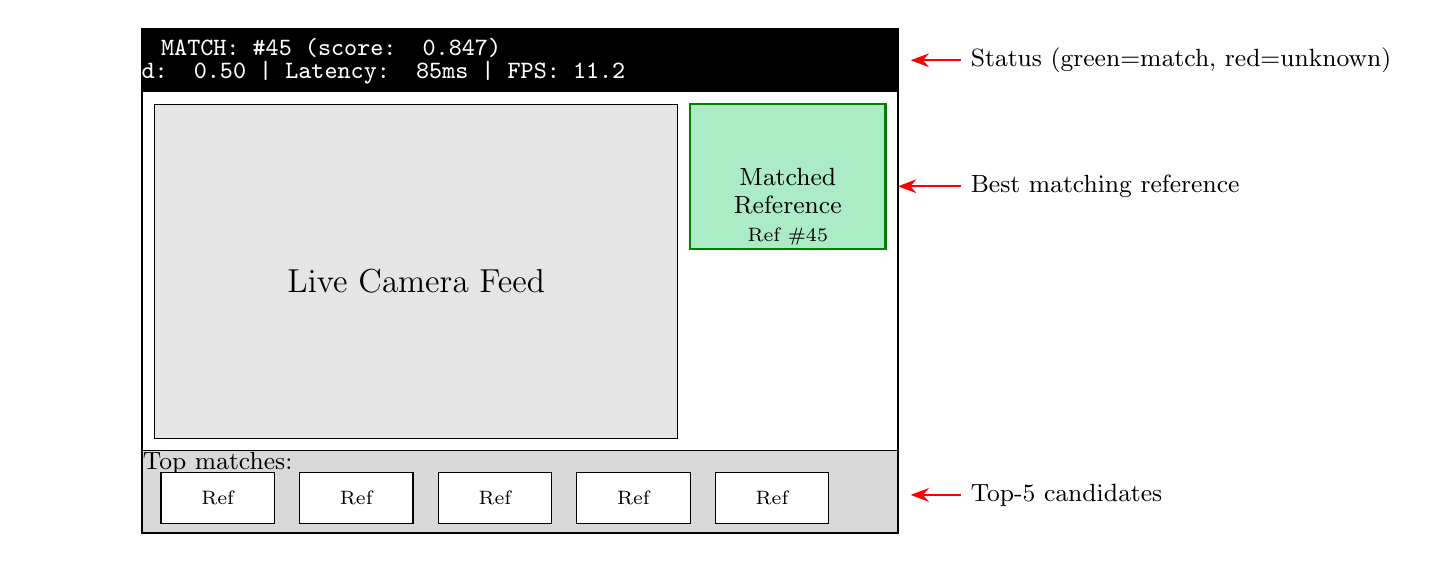
\begin{tikzpicture}[scale=0.8]
        % Main frame
        \draw[thick] (0,0) rectangle (12,8);

        % Status bar
        \draw[fill=black] (0,7) rectangle (12,8);
        \node[white, font=\ttfamily\small] at (3,7.7) {MATCH: \#45 (score: 0.847)};
        \node[white, font=\ttfamily\small] at (3,7.3) {Threshold: 0.50 | Latency: 85ms | FPS: 11.2};

        % Camera feed area
        \draw[fill=gray!20] (0.2,1.5) rectangle (8.5,6.8);
        \node at (4.35,4) {\large Live Camera Feed};

        % Reference image
        \draw[fill=lightgreen, thick, draw=green!50!black] (8.7,4.5) rectangle (11.8,6.8);
        \node[font=\small] at (10.25,5.65) {Matched};
        \node[font=\small] at (10.25,5.2) {Reference};
        \node[font=\scriptsize] at (10.25,4.7) {Ref \#45};

        % Top matches panel
        \draw[fill=gray!30] (0,0) rectangle (12,1.3);
        \node[font=\small] at (1.2,1.1) {Top matches:};

        % Thumbnails
        \foreach \i in {0,1,2,3,4} {
            \draw[fill=white] (0.3+\i*2.2,0.15) rectangle (2.1+\i*2.2,0.95);
            \node[font=\scriptsize] at (1.2+\i*2.2,0.55) {Ref};
        }

        % Annotations
        \draw[-{Stealth}, thick, red] (13,7.5) -- (12.2,7.5);
        \node[right, font=\small] at (13,7.5) {Status (green=match, red=unknown)};

        \draw[-{Stealth}, thick, red] (13,5.5) -- (12,5.5);
        \node[right, font=\small] at (13,5.5) {Best matching reference};

        \draw[-{Stealth}, thick, red] (13,0.6) -- (12.2,0.6);
        \node[right, font=\small] at (13,0.6) {Top-5 candidates};

    \end{tikzpicture}
    \caption{Live test display layout with annotations.}
\end{figure}

\newpage
% ============================================================================
\section{Testing Scenarios}
% ============================================================================

\subsection{Test Matrix}

\begin{table}[H]
    \centering
    \begin{tabular}{llcp{5cm}}
        \toprule
        \textbf{Scenario} & \textbf{Database} & \textbf{Query} & \textbf{What it Tests} \\
        \midrule
        Day $\rightarrow$ Day & Day (132) & Day (live) & Baseline recognition \\
        Day $\rightarrow$ Night & Day (132) & Night (live) & Cross-illumination robustness \\
        Night $\rightarrow$ Night & Night (223) & Night (live) & Night-only operation \\
        Night $\rightarrow$ Day & Night (223) & Day (live) & Reverse cross-illumination \\
        Combined & Day+Night & Any & Multi-condition robustness \\
        \bottomrule
    \end{tabular}
    \caption{Testing scenarios for comprehensive evaluation.}
\end{table}

\subsection{Scenario Diagrams}

\begin{figure}[H]
    \centering
    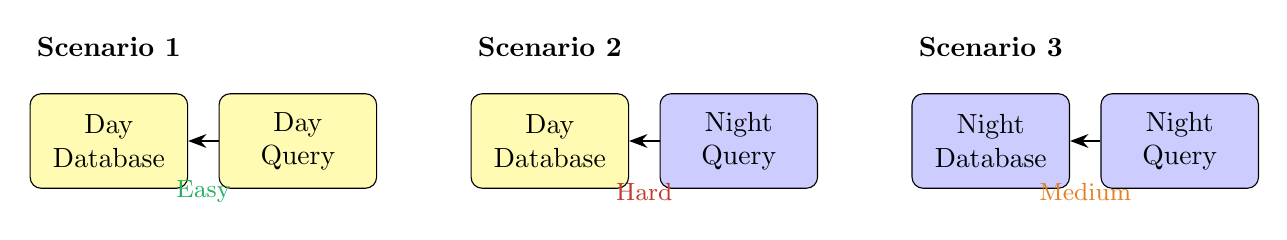
\begin{tikzpicture}[
        scale=0.8,
        box/.style={rectangle, draw, rounded corners, minimum width=2cm, minimum height=1.2cm, align=center},
        arrow/.style={-{Stealth}, thick}
    ]
        % Scenario 1: Day -> Day
        \node[font=\bfseries] at (-5, 2) {Scenario 1};
        \node[box, fill=yellow!30] (d1db) at (-5, 0.5) {Day\\Database};
        \node[box, fill=yellow!30] (d1q) at (-2, 0.5) {Day\\Query};
        \draw[arrow] (d1q) -- (d1db);
        \node[font=\small, darkgreen] at (-3.5, -0.3) {Easy};

        % Scenario 2: Day -> Night
        \node[font=\bfseries] at (2, 2) {Scenario 2};
        \node[box, fill=yellow!30] (d2db) at (2, 0.5) {Day\\Database};
        \node[box, fill=blue!20] (d2q) at (5, 0.5) {Night\\Query};
        \draw[arrow] (d2q) -- (d2db);
        \node[font=\small, darkred] at (3.5, -0.3) {Hard};

        % Scenario 3: Night -> Night
        \node[font=\bfseries] at (9, 2) {Scenario 3};
        \node[box, fill=blue!20] (d3db) at (9, 0.5) {Night\\Database};
        \node[box, fill=blue!20] (d3q) at (12, 0.5) {Night\\Query};
        \draw[arrow] (d3q) -- (d3db);
        \node[font=\small, darkorange] at (10.5, -0.3) {Medium};

    \end{tikzpicture}
    \caption{Visual comparison of testing scenarios by difficulty.}
\end{figure}

\subsection{Commands for Each Scenario}

\begin{lstlisting}[language=bash, caption=Commands for different testing scenarios]
# Scenario 1: Day -> Day (Baseline)
python live_vpr_test.py --mode build_db --data_dir data/CMUAfrica/day --db_path day_db.npz
python live_vpr_test.py --mode live_test --db_path day_db.npz --threshold 0.5
# Run during daytime

# Scenario 2: Day -> Night (Cross-illumination)
# Use same day_db.npz, run test at night
python live_vpr_test.py --mode live_test --db_path day_db.npz --threshold 0.4

# Scenario 3: Night -> Night
python live_vpr_test.py --mode build_db --data_dir data/CMUAfrica/night --db_path night_db.npz
python live_vpr_test.py --mode live_test --db_path night_db.npz --threshold 0.5
# Run during nighttime

# Scenario 4: Batch evaluation (offline, no camera needed)
python live_vpr_test.py --mode batch_eval --db_path day_db.npz --query_dir data/CMUAfrica/night
\end{lstlisting}

\newpage
% ============================================================================
\section{Evaluation Metrics}
% ============================================================================

\subsection{Key Metrics}

\begin{table}[H]
    \centering
    \begin{tabular}{lp{8cm}}
        \toprule
        \textbf{Metric} & \textbf{Description} \\
        \midrule
        Recognition Rate & Percentage of queries where similarity exceeds threshold \\
        Accuracy & Percentage of correct matches (within GT tolerance) \\
        Recall@K & Percentage of queries where true match is in top-K results \\
        Mean Similarity & Average similarity score across all queries \\
        Latency & Time to process one query (in milliseconds) \\
        \bottomrule
    \end{tabular}
    \caption{Evaluation metrics for VPR performance assessment.}
\end{table}

\subsection{Interpreting Results}

\begin{figure}[H]
    \centering
    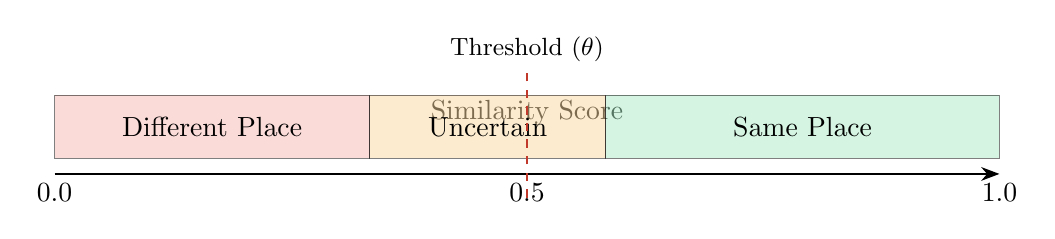
\begin{tikzpicture}
        % Similarity score scale
        \draw[thick, -{Stealth}] (0,0) -- (12,0);
        \node[below] at (0,0) {0.0};
        \node[below] at (6,0) {0.5};
        \node[below] at (12,0) {1.0};
        \node[above] at (6,0.5) {Similarity Score};

        % Zones
        \draw[fill=lightred, opacity=0.5] (0,0.2) rectangle (4,1);
        \draw[fill=lightorange, opacity=0.5] (4,0.2) rectangle (7,1);
        \draw[fill=lightgreen, opacity=0.5] (7,0.2) rectangle (12,1);

        \node at (2,0.6) {Different Place};
        \node at (5.5,0.6) {Uncertain};
        \node at (9.5,0.6) {Same Place};

        % Threshold marker
        \draw[thick, dashed, darkred] (6,-0.3) -- (6,1.3);
        \node[above, font=\small] at (6,1.3) {Threshold ($\theta$)};

    \end{tikzpicture}
    \caption{Interpreting similarity scores for place recognition.}
\end{figure}

\subsection{Tuning the Threshold}

\begin{itemize}
    \item \textbf{High threshold ($\theta > 0.6$)}: Fewer matches, higher precision, may miss correct matches
    \item \textbf{Low threshold ($\theta < 0.4$)}: More matches, higher recall, may include false matches
    \item \textbf{Recommended}: Start with $\theta = 0.5$, adjust based on your application needs
\end{itemize}

\newpage
% ============================================================================
\section{Troubleshooting}
% ============================================================================

\begin{table}[H]
    \centering
    \begin{tabular}{p{4cm}p{8cm}}
        \toprule
        \textbf{Problem} & \textbf{Solution} \\
        \midrule
        Camera not found & Try different camera IDs (0, 1, 2). Ensure phone app is running and connected. \\
        \midrule
        Low recognition rate & Lower threshold (e.g., 0.4). Check if test location matches database. \\
        \midrule
        High latency & Use GPU if available. Reduce image resolution. Try faster descriptor (AlexNet). \\
        \midrule
        Model loading fails & Ensure all dependencies installed. Check internet for model download. \\
        \midrule
        Black screen in display & Camera permissions may be blocked. Check System Preferences. \\
        \bottomrule
    \end{tabular}
    \caption{Common problems and solutions.}
\end{table}

% ============================================================================
\section{Quick Reference}
% ============================================================================

\subsection{Command Summary}

\begin{lstlisting}[language=bash, caption=Quick reference commands]
# Check camera
python live_vpr_test.py --mode check_camera --camera 0

# Build database
python live_vpr_test.py --mode build_db --data_dir <image_folder> --db_path <output.npz>

# Live test
python live_vpr_test.py --mode live_test --db_path <database.npz> --camera 0 --threshold 0.5

# Video test
python live_vpr_test.py --mode video_test --db_path <database.npz> --video <video.mp4>

# Batch evaluation
python live_vpr_test.py --mode batch_eval --db_path <database.npz> --query_dir <query_folder>
\end{lstlisting}

\subsection{Available Descriptors}

\begin{table}[H]
    \centering
    \begin{tabular}{lccc}
        \toprule
        \textbf{Descriptor} & \textbf{Dimension} & \textbf{Speed} & \textbf{Accuracy} \\
        \midrule
        CosPlace & 512 & Medium & High \\
        EigenPlaces & 512 & Medium & High \\
        NetVLAD & 4096 & Slow & High \\
        HDC-DELF & 4096 & Medium & Medium \\
        AlexNet & 64896 & Fast & Low \\
        \bottomrule
    \end{tabular}
    \caption{Comparison of available feature descriptors.}
\end{table}

\newpage
% ============================================================================
\section{Appendix: Algorithm Pseudocode}
% ============================================================================

\begin{algorithm}[H]
\caption{Live Visual Place Recognition}
\begin{algorithmic}[1]
\Require Camera stream, Database $D_{db}$, Threshold $\theta$
\Ensure Location estimates for each frame

\State \textbf{Offline Phase:}
\For{each reference image $I_i$ in training set}
    \State $d_i \gets \text{ExtractFeatures}(I_i)$
    \State $\hat{d}_i \gets d_i / \|d_i\|_2$
\EndFor
\State $D_{db} \gets [\hat{d}_1, \hat{d}_2, \ldots, \hat{d}_N]^T$
\State Save $D_{db}$ to disk

\State
\State \textbf{Online Phase:}
\While{camera is active}
    \State $I_q \gets \text{CaptureFrame}()$
    \State $d_q \gets \text{ExtractFeatures}(I_q)$
    \State $\hat{d}_q \gets d_q / \|d_q\|_2$
    \State $S \gets D_{db} \cdot \hat{d}_q^T$ \Comment{Similarity scores}
    \State $k^* \gets \text{argmax}(S)$
    \If{$S_{k^*} > \theta$}
        \State \Return Location $k^*$ with confidence $S_{k^*}$
    \Else
        \State \Return Unknown location
    \EndIf
\EndWhile
\end{algorithmic}
\end{algorithm}

% ============================================================================
\section{Conclusion}
% ============================================================================

This guide provides a complete framework for deploying Visual Place Recognition on the CMU-Africa campus dataset. The system supports:

\begin{itemize}
    \item Real-time localization using smartphone cameras
    \item Multiple testing scenarios (day/night, cross-illumination)
    \item Flexible evaluation with adjustable thresholds
    \item Batch processing for offline analysis
\end{itemize}

For questions or issues, contact the development team or refer to the project repository.

\vspace{1cm}
\hrule
\vspace{0.5cm}
\textit{Document generated: March 2026}\\
\textit{VPR Tutorial Repository: stschubert/VPR\_Tutorial}

\end{document}
